% =====================================================================
%  TomaNet-C (classification), drawn with the real PlotNeuralNet layer
%  library (Box / Ball) -- one solid 3D tile per operation.
%  IMPORTANT: depth is kept small relative to width on every box. The
%  library's -east/-west/-nearwest/-neareast anchors sit at the box's
%  own x-extent at z=0 / z=+depth/2; if depth is comparable to (or
%  larger than) width, that x-extent is a thin sliver buried inside the
%  parallelogram the depth-skew draws, so connector lines visibly cut
%  into the box instead of touching its edge. Keeping width notably
%  larger than depth (checked empirically) puts -neareast/-nearwest
%  right at the visible edge.
%  Stem + backbone pics are byte-for-byte the same as fig_tomanet_d.tex.
% =====================================================================
\documentclass[border=12pt, multi, tikz]{standalone}
\usepackage{import}
\subimport{./layers/}{init}
\usetikzlibrary{positioning,3d,calc}
% =====================================================================
%  tomanet_palette.tex -- one colour per architectural role, shared by
%  fig_tomanet_c.tex and fig_tomanet_d.tex so a shared module (the stem
%  and backbone) keeps the exact same colour in both figures. That
%  visual identity IS the point: TomaNet-C and TomaNet-D use a
%  byte-identical trunk (layers 0-8) and only the colours after the
%  trunk change.
% =====================================================================
\definecolor{tStem}   {RGB}{243,203,150}  % stem convs             sand
\definecolor{tStemP}  {RGB}{253,240,222}  % stem panel
\definecolor{tTrunk}  {RGB}{150,196,140}  % TomaLayer stages        leaf green
\definecolor{tTrunkP} {RGB}{232,244,227}  % trunk panel
\definecolor{tBlkA}   {RGB}{120,175,190}  % RepPConv / spatial      teal
\definecolor{tBlkB}   {RGB}{150,150,200}  % CoordAtt                periwinkle
\definecolor{tNeck}   {RGB}{ 90,110,175}  % TomaLayer, neck (e=1.0) deep slate blue
\definecolor{tNeckP}  {RGB}{231,236,247}  % neck panel
\definecolor{tStruct} {RGB}{200,200,200}  % structural ops: upsample / concat -- not a learned layer, so deliberately neutral grey
\definecolor{tHeadC}  {RGB}{210,110,90}   % classify head           tomato red
\definecolor{tHeadCP} {RGB}{250,231,225}  % classify head panel
\definecolor{tHeadD}  {RGB}{210,110,90}   % detect heads            tomato red (same family: both are "the answer")
\definecolor{tHeadDP} {RGB}{250,231,225}  % detect head panel
\definecolor{tLine}   {RGB}{ 90,100,95}   % connector
\definecolor{tRule}   {RGB}{200,206,200}  % separators

% ---- PlotNeuralNet 3D-tile band colours (darker shade of each block's
% own hue, used for RightBandedBox's second face -- e.g. "the BN+act
% half" or "the attention half" of a two-part operation) -------------
\colorlet{tStemBand}  {tStem!60!black}
\colorlet{tTrunkBand} {tTrunk!60!black}
\colorlet{tNeckBand}  {tNeck!60!black}
\colorlet{tHeadCBand} {tHeadC!60!black}
\colorlet{tHeadDBand} {tHeadD!60!black}
\colorlet{tBlkABand}  {tBlkA!60!black}
\colorlet{tBlkBBand}  {tBlkB!60!black}
\definecolor{tBlkSum} {RGB}{190,140,150}  % residual / concat ball    dusty rose


\begin{document}
\begin{tikzpicture}[font=\Large]
\tikzstyle{connection}=[ultra thick,every node/.style={sloped,allow upside down},draw=\edgecolor,opacity=0.7]
\tikzstyle{caplabel}=[text width=4.0cm,text centered,font=\Large]

% ----------------------------------------------------------------
% input image plane
% ----------------------------------------------------------------
\node[canvas is zy plane at x=0] (input) at (-2.8,0,0)
      {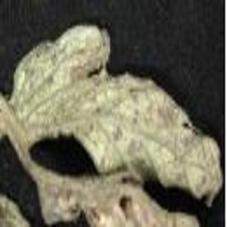
\includegraphics[width=3.2cm,height=3.2cm]{cls_leaf.png}};
\node[caplabel] at (-2.8,-3.0,0) {input leaf, $224^2{\times}3$};

% ----------------------------------------------------------------
% stem: two strided convs, each its own tile
% ----------------------------------------------------------------
\pic[shift={(0,0,0)}] at (0,0,0)
     {Box={name=st1,caption=Conv $3{\times}3$/2,%
       xlabel={{"64",""}},zlabel=$112^2$,fill=tStem,opacity=0.85,%
       height=44,width=18,depth=9}};

\pic[shift={(3.6,0,0)}] at (st1-east)
     {Box={name=st2,caption=Conv $3{\times}3$/2,%
       xlabel={{"128",""}},zlabel=$56^2$,fill=tStem,opacity=0.85,%
       height=34,width=20,depth=9}};

% ----------------------------------------------------------------
% backbone: 4 TomaLayer stages, byte-identical to fig_tomanet_d.tex
% ----------------------------------------------------------------
\pic[shift={(3.8,0,0)}] at (st2-east)
     {Box={name=s2,caption=TomaLayer$\times2$,%
       xlabel={{"128",""}},zlabel=$56^2$,fill=tTrunk,opacity=0.85,%
       height=34,width=22,depth=9}};

\pic[shift={(4.0,0,0)}] at (s2-east)
     {Box={name=s3,caption=TomaLayer$\times4$,%
       xlabel={{"256",""}},zlabel=$28^2$,fill=tTrunk,opacity=0.85,%
       height=24,width=24,depth=9}};

\pic[shift={(4.0,0,0)}] at (s3-east)
     {Box={name=s4,caption=TomaLayer$\times4$,%
       xlabel={{"512",""}},zlabel=$14^2$,fill=tTrunk,opacity=0.85,%
       height=16,width=26,depth=9}};

\pic[shift={(4.0,0,0)}] at (s4-east)
     {Box={name=s5,caption=TomaLayer$\times2$,%
       xlabel={{"1024",""}},zlabel=$7^2$,fill=tTrunk,opacity=0.85,%
       height=9,width=28,depth=8}};

% ----------------------------------------------------------------
% classification head: GAP (ball) -> FC+softmax (box)
% ----------------------------------------------------------------
\pic[shift={(3.4,0,0)}] at (s5-east)
     {Ball={name=gap,caption=global avg pool,fill=tHeadC,opacity=0.7,%
       radius=2.6,logo={avg}}};

\pic[shift={(3.0,0,0)}] at (gap-east)
     {Box={name=fc,caption=FC + softmax,%
       xlabel={{"nc",""}},fill=tHeadC,opacity=0.85,%
       height=10,width=16,depth=8}};

% ----------------------------------------------------------------
% output image plane + predicted label
% ----------------------------------------------------------------
\node[canvas is zy plane at x=0] (output) at ($(fc-east)+(3.2,0,0)$)
      {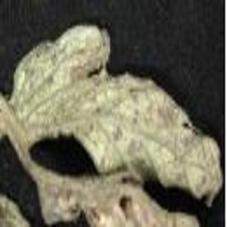
\includegraphics[width=3.2cm,height=3.2cm]{cls_leaf.png}};
\node[caplabel] at ($(fc-east)+(3.2,-3.0,0)$)
      {\texttt{bacterial\_spot}, $0.50$};

% ----------------------------------------------------------------
% connections
% ----------------------------------------------------------------
\draw[connection] (input.east)  -- node{\midarrow} (st1-nearwest);
\draw[connection] (st1-neareast)-- node{\midarrow} (st2-nearwest);
\draw[connection] (st2-neareast)-- node{\midarrow} (s2-nearwest);
\draw[connection] (s2-neareast) -- node{\midarrow} (s3-nearwest);
\draw[connection] (s3-neareast) -- node{\midarrow} (s4-nearwest);
\draw[connection] (s4-neareast) -- node{\midarrow} (s5-nearwest);
\draw[connection] (s5-neareast) -- node{\midarrow} (gap-west);
\draw[connection] (gap-east)    -- node{\midarrow} (fc-nearwest);
\draw[connection] (fc-neareast) -- node{\midarrow} (output.west);

% ----------------------------------------------------------------
% TomaBlock inset: the one brick reused inside every TomaLayer stage,
% at every scale, in both TomaNet-C and TomaNet-D. One tile per nn
% module in tomanet/modules.py, in exact forward() order.
% ----------------------------------------------------------------
\node[caplabel,text width=13cm,font=\Large\bfseries] at ($(s3-anchor)+(0,-6.8,0)$)
     {TomaBlock -- the shared brick inside every TomaLayer};

\pic[shift={(0,-9.6,0)}] at (s2-anchor)
     {Box={name=tb1,caption={RepPConv $3{\times}3$, $1/4$ ch},%
       xlabel={{"3$\to$1",""}},fill=tBlkA,opacity=0.85,%
       height=15,width=17,depth=8}};

\pic[shift={(3.2,0,0)}] at (tb1-east)
     {Box={name=tb2,caption=$1{\times}1$ expand $\times2$,%
       xlabel={{"exp",""}},fill=tBlkA,opacity=0.7,%
       height=15,width=17,depth=8}};

\pic[shift={(3.2,0,0)}] at (tb2-east)
     {Box={name=tb3,caption=DWConv $k{\times}k$,%
       xlabel={{"dw",""}},fill=tBlkB,opacity=0.85,%
       height=15,width=17,depth=8}};

\pic[shift={(3.2,0,0)}] at (tb3-east)
     {Box={name=tb4,caption=CoordAtt,%
       xlabel={{"attn",""}},fill=tBlkB,opacity=0.7,%
       height=15,width=17,depth=8}};

\pic[shift={(3.2,0,0)}] at (tb4-east)
     {Box={name=tb5,caption=$1{\times}1$ project,%
       xlabel={{"proj",""}},fill=tBlkA,opacity=0.85,%
       height=15,width=17,depth=8}};

\pic[shift={(2.8,0,0)}] at (tb5-east)
     {Ball={name=tbsum,caption={residual, $c_1{=}c_2$},fill=tBlkSum,%
       opacity=0.7,radius=2.2,logo=$+$}};

\draw[connection] (tb1-neareast) -- node{\midarrow} (tb2-nearwest);
\draw[connection] (tb2-neareast) -- node{\midarrow} (tb3-nearwest);
\draw[connection] (tb3-neareast) -- node{\midarrow} (tb4-nearwest);
\draw[connection] (tb4-neareast) -- node{\midarrow} (tb5-nearwest);
\draw[connection] (tb5-neareast) -- node{\midarrow} (tbsum-west);
\draw[connection,densely dashed] (tb1-nearwest) -- ++(0,-3.8,0) -| (tbsum-south);
\draw[connection,densely dashed] (s2-south) -- ++(0,-2.4,0) -| (tb1-north);

\end{tikzpicture}
\end{document}
